\begin{figure}[!t]
\begin{center}
\begin{tabular}{ccc}
\hspace{-0.3cm}\includegraphics[width=0.33\textwidth,height=9cm]{datasetB.eps}&
\hspace{-0.4cm}\includegraphics[width=0.33\textwidth,height=9cm]{datasetC.eps}&
\hspace{-0.4cm}\includegraphics[width=0.33\textwidth,height=9cm]{datasetA.eps}\\
\textbf{(a)}&\textbf{(b)}&\textbf{(c)}\\
\end{tabular}
\caption[Example of urban images for driving scenes]{Example of urban images used in our experiments. a)
Images from CamVid~\cite{CamVidBBDD:PRL2008} dataset (day on the
left and dusk on the right); b) Images from
KITTI~\cite{Fritsch2013ITSC} road-dataset and; c) Collection of
images retrieved from Google.} \label{fig:datasets}
\end{center}
\vspace{-5mm}
\end{figure}
\section{Experimental Analysis}
\label{sec:experiments}

In this section, we conduct several experiments to demonstrate the
benefits of incorporating our image transformation method in general
state-of-the-art semantic segmentation tools. More precisely, we
consider two different setups: (i) the training set used to create
the semantic segmentation model is available and (ii) where the
training set is not available. We also test the advantages of
using a one-to-$K$ matching. Experiments are
conducted on three state-of-the-art urban datasets, where the
visual conditions are largely different, using three different
semantic labelling frameworks: Photo Pop-up (Hoiem
\etal~\cite{HoiemIJCV:2007}), a recent work by Yang
\etal~\cite{Make3dCVPR:2014}, and Darwin (Gould
\etal~\cite{DARWIN}). The first two approaches are existing
algorithms for recovering the layout of a scene and are used as
they are with no retraining. Both approaches were originally
trained with generic images from generic environments. The last
method is the framework introduced in~\cite{DARWIN}. In this case,
we retrain the classifier with domain specific images (urban
images) using a non-overlapping subsets of images from each
dataset depending on the experiment.



\subsection{Datasets \& classes}
\label{subsect:datasets} Experiments are conducted on three
datasets. First, the Cambridge-driving Labeled Video Database
(CamVid)~\cite{CamVidBBDD:PRL2008}, a publicly available
collection of videos captured in the UK from the perspective of a
driving automobile with ground truth labels that associate each
pixel with one of $32$ semantic classes. This dataset is divided
in four sequences, i.e., 1TP, 6R0, 16E5 and Seq05SV. The first one
consists of dark images, simulating dusk conditions, while the
remaining are gathered in daytime conditions, as shown
in~\subfig{fig:datasets}{\textbf{(a)}}. In our experiments we transform the
$32$ semantic classes into $3$ general classes: Sky (S),  Ground
plane (G) and Vertical obstacles (V).

Second, we use the also publicly available KITTI
dataset~\cite{KITTI}. KITTI also consists of images
acquired from a moving car in Karlsruhe,
Germany~\subfig{fig:datasets}{\textbf{(b)}}. The ground truth for
this dataset has been generated by manually annotating the $323$
images images of the KITTI-Road Benchmark~\cite{Fritsch2013ITSC}.
Finally, we collect a set of images from Google showing
particularly challenging scenarios such as night time and sunset
situations as shown in~\subfig{fig:datasets}{\textbf{(c)}}.
\begin{figure}[!t]
    \centering
    %\vspace{-1mm}
    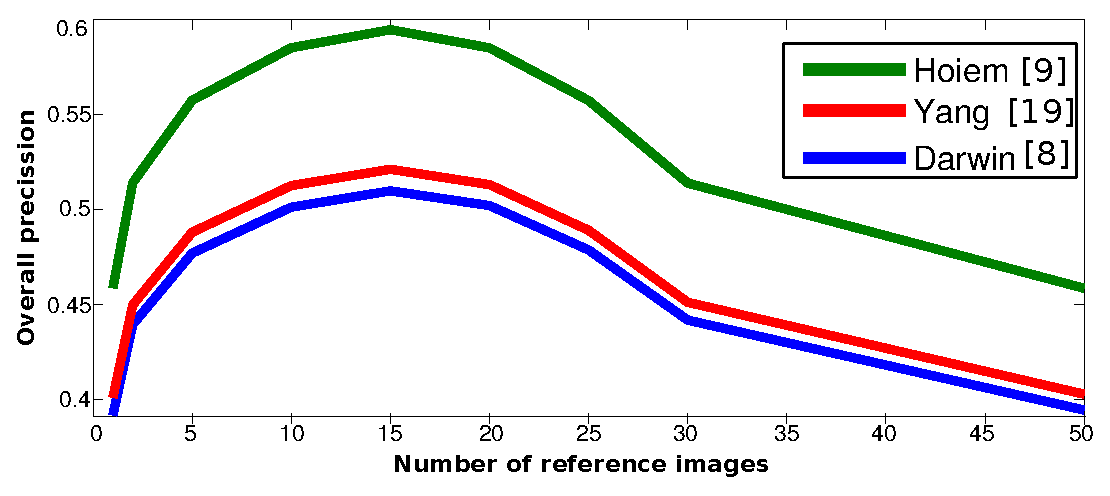
\includegraphics[scale=0.6]{Ks.eps}
    \vspace{-2mm}
    \caption[K-selection, overall performance analysis]{Overall performance with respect to $K$, the number of reference images, on the CamVid dataset.}
    \label{fig:Ks}
    \vspace{2mm}
\end{figure}
%
%\subsection{Semantic Labelling Frameworks}
%Experiments are conducted using three publicly available
%algorithms: Photo Pop-up (Hoiem \etal~\cite{HoiemIJCV:2007}), a
%recent work by Yang \etal~\cite{Make3dCVPR:2014}, and Darwin
%(Gould \etal~\cite{DARWIN}). The first two approaches are existing
%algorithms for recovering the layout of a scene and are used as
%they are with no retraining. Both approaches were originally
%trained with generic images from generic environments. The last
%method is the framework introduced in~\cite{DARWIN}. In this case,
%we retrain the classifier with domain specific images (road
%images) using a non-overlapping subset from CamVid or KITTI
%depending on the experiment.

%The set of experiments reveals that the preprocessing step improves the performance of existing classifiers in random consitions. To validate the proposal we use three the frameowrks shown in~\fig{} and we consider three instances of classifiers: the approach for recovering the 3D scene layout in~\cite{}, make3D and finally we consider a textoonbost classifier as described in~\cite{}. The first two approaches are used without retraining and represent two different conditions. The first one aims at recovering the layout of a road scene and the neural network was originally trained in using road scenes. The second approach is targeted to general images therefore dealing with the specific conditions of real driving situations is more complicated. Finally, we retrain the approach in~\cite{} using images from ...

\subsection{Quantitative and Qualitative Evaluation}
\textbf{First experiment:} We start by assessing the variation in
performance of the three semantic labellers, when the images are
adapted following our approach. Quantitative evaluations in terms
of Overall Precision (\textbf{OP}) and Per-class Average
(\textbf{PC})~\cite{Ladicky:2013} on the KITTI and CamVid are summarized in
Table~\ref{tab:results1} and Table~\ref{tab:results2},
respectively.

As shown in Table~\ref{tab:results1}, on the KITTI dataset, the
impact of transferring images is not significant, even leading to
some slight loss of performance for Yang's method and Darwin. This
is mainly due to the good conditions of the images. However, as
shown in Table~\ref{tab:results2}, when the experiment is carried
out on the CamVid dataset, the situation is quite different. For
the dusk sequence (1TP) the accuracy of all three methods
increases significantly, with more than $20$ points of improvement
for Hoiem and, $13$ and $8$ points for Yang and Darwin,
respectively. Qualitative examples of this improvement are shown
in Fig.~\ref{fig:1TP}\textbf{(a)}. For the remaining sequences, acquired in
daytime, this improvement is reduced, and only Hoiem and Yang
present some slight benefits. Again, this is mainly due to the
already existing similarities in the color properties of the
training and the testing images.

The impact of our method is now illustrated using the set of
challenging images from Google Images showing night time and
sunset situations. Qualitative results of this experiment are
presented in Fig.~\ref{fig:1TP}\textbf{(b)}. As shown, although the
resulting labelling is far from perfect, the improvement is
notorious. This is specially true for Hoiem and Darwin frameworks,
which achieve the best results. From these quantitative and
qualitative evaluations, we can conclude that including our image
adaptation method improves the performance of semantic labellers
specially in challenging situations not seen during the training
stage.

\begin{table}[!t]
\caption[Quantitative evaluations of three semantic labelling
frameworks on the KITTI dataset.]{Quantitative evaluations of three semantic labelling
frameworks on the KITTI dataset. Adapted refers to performance
when our image transformation is included in the pipeline.}
\centering
%\resizebox{\columnwidth}{!}{%
%\scriptsize
%\tabcolsep=0.06cm
\begin{tabular}{|c|c|c|}
\cline{2-3}\noalign{\vskip 1pt}
\multicolumn{1}{c|}{ } & \multicolumn{2}{|c|}{KITTI Road Dataset}\\
\cline{2-3}\noalign{\vskip 1pt}
\multicolumn{1}{c|}{ } & \textbf{OP} & \textbf{PC}\\
\hline
Hoiem~\cite{HoiemIJCV:2007} Original & 0.67 & 0.65 \\
\hline
Hoiem~\cite{HoiemIJCV:2007} Transformed & 0.67 & 0.65 \\
\hline
Yang~\cite{Make3dCVPR:2014} Original & 0.62 & 0.57 \\
\hline
Yang~\cite{Make3dCVPR:2014} Transformed & 0.61 & 0.57 \\
\hline
Darwin~\cite{DARWIN} (Camvid) Original & 0.67 & 0.62 \\
\hline
Darwin~\cite{DARWIN} (Camvid) Transformed & 0.64 & 0.62 \\
\hline
\end{tabular}%
%}
\label{tab:results1} \vspace{-1mm}
\end{table}

\begin{table}[t]
\caption[Quantitative evaluations of three semantic labelling
frameworks on the CamVid dataset.]{Quantitative evaluations of three semantic labelling
frameworks on the CamVid dataset. Adapted refers to performance
when our image transformation is included in the pipeline.}
\centering
\resizebox{0.9\columnwidth}{!}{%
%\scriptsize
%\tabcolsep=0.06cm
\begin{tabular}{|c|c|c|c|c|c|c|c|c|}
\cline{2-9}\noalign{\vskip 1pt}
\multicolumn{1}{c|}{ } & \multicolumn{8}{|c|}{CamVid Dataset}\\
\cline{2-9}\noalign{\vskip 1pt}
\multicolumn{1}{c|}{ } & \multicolumn{2}{|c|}{1TP} & \multicolumn{2}{|c|}{6R0} & \multicolumn{2}{|c|}{16E5} & \multicolumn{2}{|c|}{05SV}\\
\cline{2-9}\noalign{\vskip 1pt}
\multicolumn{1}{c|}{ } & \textbf{OP} & \textbf{PC} & \textbf{OP} & \textbf{PC} & \textbf{OP} & \textbf{PC} & \textbf{OP} & \textbf{PC}\\
\hline
Hoiem~\cite{HoiemIJCV:2007} Original & 0.61 & 0.38 &  \textbf{0.85} & \textbf{0.65} & 0.87 & 0.67 &   0.87 & 0.64\\
\hline
Hoiem~\cite{HoiemIJCV:2007} Transformed & \textbf{0.83} & \textbf{0.65} &     0.84 & 0.63 &   \textbf{0.89} & \textbf{0.68} &     0.87 & 0.64\\
\hline
Yang~\cite{Make3dCVPR:2014} Original & 0.58 & 0.35 & 0.87 & 0.68 & 0.84 & 0.61 & 0.91 & 0.70\\
\hline
Yang~\cite{Make3dCVPR:2014} Transformed & \textbf{0.71} & \textbf{0.51} & 0.87 & 0.68 & \textbf{0.85} & \textbf{0.63} & 0.91 & \textbf{0.71}\\
\hline
Darwin~\cite{DARWIN} (KITTI) Original & 0.68 & 0.61 & 0.84 & 0.77 & \textbf{0.93} & \textbf{0.90} & \textbf{0.89} & \textbf{0.81}\\
\hline
Darwin~\cite{DARWIN} (KITTI) Transformed & \textbf{0.76} & \textbf{0.71} & 0.84 & 0.77 & 0.91 & 0.84 & 0.85 & 0.73\\
\hline
\end{tabular}%
}  \label{tab:results2} %\vspace{-5mm}
\vspace{4mm}
\end{table}


\begin{table}[t]
\caption[Influence of including temporal coherence on the
CamVid dataset.]{Influence of including temporal coherence (TCT) on the
CamVid dataset. As shown, our approach for exploiting correlation
between consecutive frames improves the performance of semantic
labellers.} \centering
\resizebox{0.9\columnwidth}{!}{%
%\scriptsize
%\tabcolsep=0.06cm
\begin{tabular}{|c|c|c|c|c|c|c|c|c|}
\cline{2-9}\noalign{\vskip 1pt}
\multicolumn{1}{c|}{ } & \multicolumn{8}{|c|}{CamVid Dataset}\\
\cline{2-9}\noalign{\vskip 1pt}
\multicolumn{1}{c|}{ } & \multicolumn{2}{|c|}{1TP} & \multicolumn{2}{|c|}{6R0} & \multicolumn{2}{|c|}{16E5} & \multicolumn{2}{|c|}{05SV}\\
\cline{2-9}\noalign{\vskip 1pt}
\multicolumn{1}{c|}{ } & \textbf{OP} & \textbf{PC} & \textbf{OP} & \textbf{PC} & \textbf{OP} & \textbf{PC} & \textbf{OP} & \textbf{PC}\\
\hline
Hoiem~\cite{HoiemIJCV:2007} Transformed & 0.82 & 0.64 & 0.83 & 0.63 & 0.89 & 0.68 & 0.87 & 0.64\\
\hline
Hoiem~\cite{HoiemIJCV:2007} Transformed-TCT & \textbf{0.83} & \textbf{0.65} &     \textbf{0.84} & 0.63 & 0.89 & {0.68} &  0.87 & 0.64\\
\hline
Darwin~\cite{DARWIN} (KITTI) Transformed & 0.75 & 0.71 & 0.76 & 0.65 & 0.90 & 0.81 & 0.85 & 0.73\\
\hline
Darwin~\cite{DARWIN} (KITTI) Transformed-TCT & \textbf{0.76} & {0.71} & \textbf{0.84} & \textbf{0.77} & \textbf{0.91} & \textbf{0.84} & 0.85 & 0.73\\
\hline
\end{tabular}%
} \label{tab:results3}
\vspace{7mm}
\end{table}

\textbf{Second experiment:} The goal of this experiment is
evaluating the influence of varying the parameter $K$ (number of
representative images) during the dictionary creation stage. To
this end, we test the overall precision (OP) of the labellers with
respect to different values of $K$ on the CamVid dataset. As shown
in Fig.~\ref{fig:Ks}, having several reference images for the
transfer is important. Moreover, for these datasets, the optimal
value is $K \approx 15$, for the three classifiers. From
these results we can conclude that the proposed one-to-$K$ transfer strategy outperforms the one-to-one strategy by Reinhard.

\textbf{Third experiment:} The goal of this experiment is
analyzing the impact of exploiting the temporal consistency in the
transfer (TCT) process when dealing with video streams.
Table~\ref{tab:results3} summarizes the performance variations
when TCT is included on the CamVid dataset. From this results, we
can conclude that considering temporal coherence outperforms still
images. This improvement is specially relevant for Darwin in
sequence 6R0, increasing the accuracy in $8$ points.


\begin{figure*}[!t]
    \centering
    %\vspace{-1mm}
    \includegraphics[width=1\textwidth]{mix.eps}
    \vspace{-5mm}
    \caption[Qualitative results for semantics transference]{\textbf{(a)} Qualitative results on the CamVid dusk dataset (1TP). As shown, labelling results are significantly better when images are adapted using the proposed method. \textbf{(b)} Qualitative results on the set of challenging images retrieved from Google. As shown, labelling results are significantly better when images are adapted using the proposed method.}
    \label{fig:1TP}
    \vspace{5mm}
\end{figure*}
